\documentclass[paper=a4, fontsize=10pt]{jlreq}

\usepackage{amsmath, amssymb}
\usepackage{enumerate}
\usepackage{tikz}
\usepackage{listings, xcolor}
\usepackage{graphicx}
\usepackage{subcaption}

\lstset{
  basicstyle = {\ttfamily},
  frame = {tbrl},
  breaklines = true,
  numbers = left,
  showspaces = false,
  showstringspaces = false,
  showtabs = false,
  keywordstyle = \color{blue},
  commentstyle = {\color[HTML]{1AB91A}},
  identifierstyle = \color{black},
  stringstyle = \color{brown},
  captionpos = t
}

\title{情報学群実験第3 NetworkSimulator}
\author{学籍番号 1280391 \\ 細川 夏風}
\date{\today}

\begin{document}

\maketitle

\section{UDP通信における帯域幅とキューサイズの影響}
\subsection{方法}
\texttt{UDP}通信の帯域幅，及びキューサイズを変更しその際のスループット，パケット損失率を観察する．また，この時の帯域幅は$1$\texttt{Mb}から$1$\texttt{Mb}ずつ上昇させ，キューサイズは$2$\texttt{KB}から$32$\texttt{KB}まで上昇させる．

\subsection{結果}
上記実験の結果を以下に示す．

\begin{figure}[htbp]
  \begin{subfigure}{0.48\columnwidth}
    \centering
    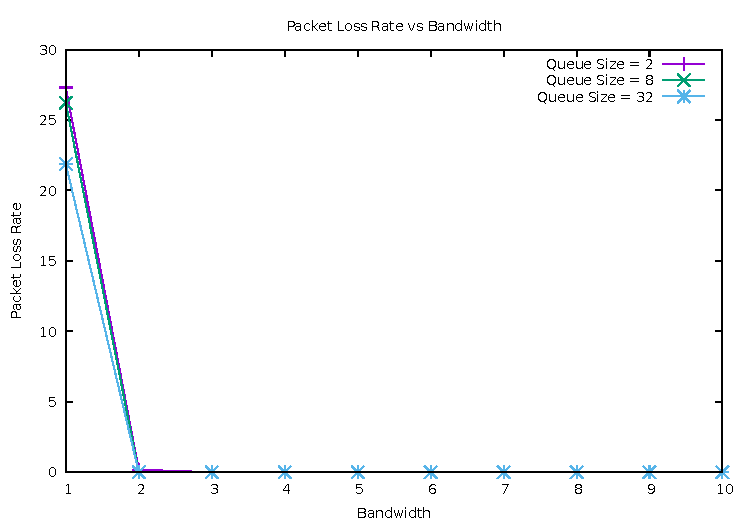
\includegraphics[width=\linewidth]{packet_loss(1-2).pdf}
    \caption{パケットロス(1-2)}
    \label{fig:loss12}
  \end{subfigure}
  \hfill
  \begin{subfigure}{0.48\columnwidth}
    \centering
    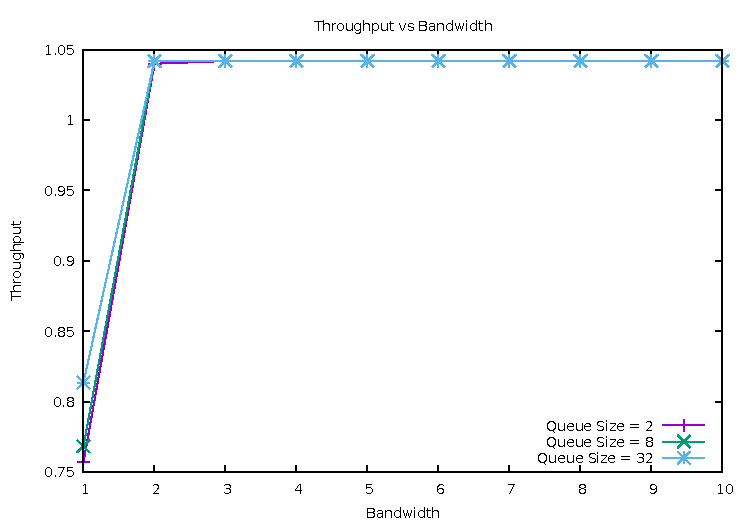
\includegraphics[width=\linewidth]{throughput(1_2).pdf}
    \caption{スループット(1-2)}
    \label{fig:tp12}
  \end{subfigure}
  \caption{ネットワーク計測結果の比較}
  \label{fig:comparison}
\end{figure}

\subsection{考察}
上記の$2$図からわかることとして少量のキューサイズであったも上昇の影響は大きいということがわかる．

\section{TCP通信における帯域幅の影響とUDP通信との比較}
\subsection{方法}
\texttt{TCP}通信の帯域幅を初期値$0.5$\texttt{Mb}から最大値$10$\texttt{Mb}まで$0.5$\texttt{Mb}ずつ上昇させスループット，パケット損失率を観察する．

\subsection{結果}
\subsubsection*{TCP通信}

% --- (1-3)のPDFファイルを横に並べる ---
\begin{figure}[htbp]
  \begin{subfigure}{0.48\columnwidth}
    \centering
    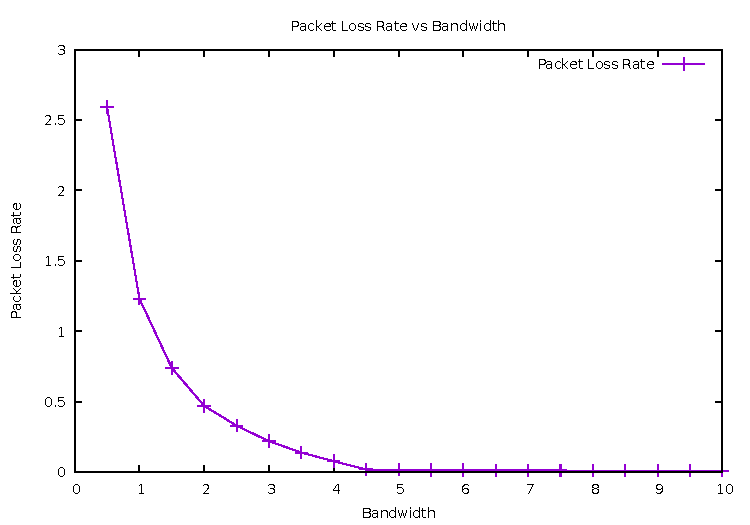
\includegraphics[width=\linewidth]{packet_loss(1-3).pdf}
    \caption{パケットロス(1-3)}
    \label{fig:loss13}
  \end{subfigure}
  \hfill
  \begin{subfigure}{0.48\columnwidth}
    \centering
    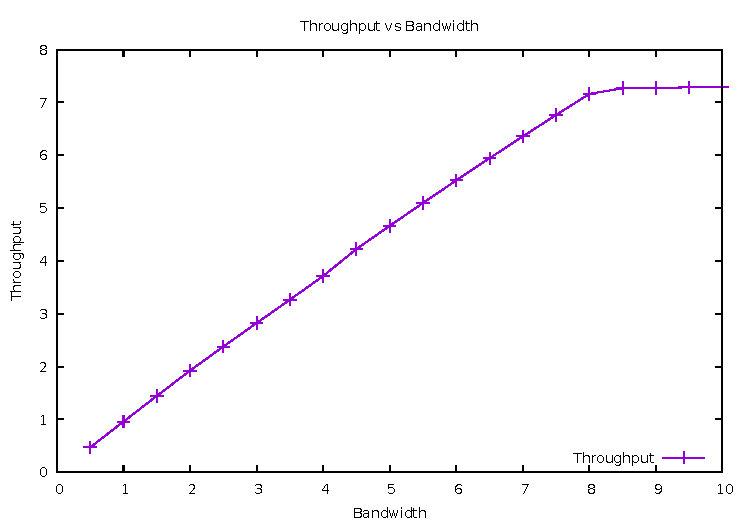
\includegraphics[width=\linewidth]{throughput(1-3).pdf}
    \caption{スループット(1-3)}
    \label{fig:tp13}
  \end{subfigure}
  \caption{TCP通信の計測結果(1-3)}
  \label{fig:tcp13}
\end{figure}

\newpage

\subsubsection*{UDP通信}

% --- UDP.pdfファイルを横に並べる ---
\begin{figure}[htbp]
  \begin{subfigure}{0.48\columnwidth}
    \centering
    % ※コンパイルエラーが出る場合は.pdf2pdfで変換してから {PACKET_LOSS.pdf} に書き換えてください
    
\includegraphics[width=\linewidth]{PACKET_LOSS.pdf}
    \caption{パケットロス(UDP)}
    \label{fig:loss_udp}
  \end{subfigure}
  \hfill
  \begin{subfigure}{0.48\columnwidth}
    \centering
    % ※コンパイルエラーが出る場合は.pdf2pdfで変換してから {THROUGHPUT.pdf} に書き換えてください
    
\includegraphics[width=\linewidth]{THROUGHPUT.pdf}
    \caption{スループット(UDP)}
    \label{fig:tp_udp}
  \end{subfigure}
  \caption{UDP通信の計測結果}
  \label{fig:udp}
\end{figure}

\subsection{考察}
以上の$2$図から，スループットには大幅な変化は無いことがわかる．これはスループットが単位時間あたりにおける通信量であるため，データ量や転送方法の影響を受けにくいことが理由として挙げられる．パケットロスについては\texttt{TCP}通信の帯域幅$1 \sim 3$について大幅に減少していることとパケットロス自体が少ないことがわかる．これは\texttt{TCP}の持つ輻輳制御が理由であると考えられる．\texttt{TCP}には輻輳制御があり，パケットロスを減らす役割を持つ．そのため，通信に輻輳が検知されるとパケットの量を調整しパケットロスを減らしてくれるのだ．初期がパケットロスが\texttt{TCP}通信では多いのはやはり，帯域幅が小さすぎるからであると考える．

\newpage

\section{追加データ}
\texttt{TCP}通信に含まれるデータからシーケンス番号(\texttt{seqno})，輻輳ウィンドウ(\texttt{cwnd})，スロースタート閾値(\texttt{ssthresh})の値を抜き出して図に示す．
\subsection{結果}
\begin{figure}
  \centering
  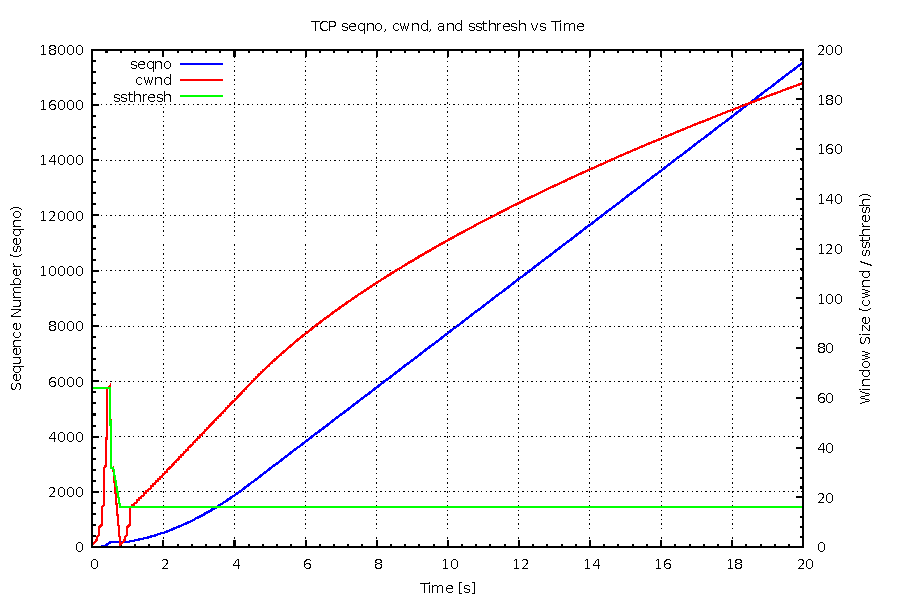
\includegraphics[width=\linewidth]{tcp_combined.pdf}
  \caption{\texttt{TCP}通信におけるシーケンス番号，輻輳ウィンドウ，スロースタート閾値の遷移}
  \label{fig:add_figure}
\end{figure}

\subsection{考察}
図\ref{fig:add_figure}から，シーケンス番号の値，輻輳ウィンドウのサイズが大きく減少している時間が存在している．これはおそらくタイムアウトが起こった状況であることがわかる．しかし，あらゆる手を尽くしてこのタイムアウト(不確定)のことについて考えて見たが確証のあるデータは得られなかった．ただ，同一のシーケンス番号の\texttt{ACK}が通常を遥かに超える回数各ノードに流れていることがわかった．これは本来ありえないことであり．これがタイムアウトの手がかかりになっていると考えられる．また，このデータから輻輳ウィンドウを超えると定数倍，正確には$\frac{1\text{segment(Byte)}}{\text{cwnd}} \times 1\text{segment(Byte)}_{\cite{TCP_IP}}$の値になっていることがわかる．

\vspace{\baselineskip}

また，今回実験データの収集のために用いたプログラムは付録に掲載している．

\begin{thebibliography}{99}
  \bibitem{TCP_IP} マスタリングTCP/IP 入門篇 第5版，竹下隆史・村山公保・荒井透・苅田幸雄，株式会社オーム社，平成26年5月20日
\end{thebibliography}

% ここから付録の開始
\appendix
\section{付録：シェルスクリプト}

\subsection{パケット処理スクリプト}
% \lstinputlisting で外部のテキストファイルをそのまま読み込めます
\lstinputlisting[caption={packet2.sh}, label={src:packet2}]{packet2.sh}

\subsection{TCPパケット処理スクリプト}
% キャプション内のアンダースコア(_)は \_ とエスケープしています（後述）
\lstinputlisting[caption={packet\_TCP.sh}, label={src:packet_tcp}]{packet_TCP.sh}

\end{document}
